%!TEX root = main.tex

\section{Motivation}
\label{sec:motivate}

\begin{figure*}[t!]
  \centering
  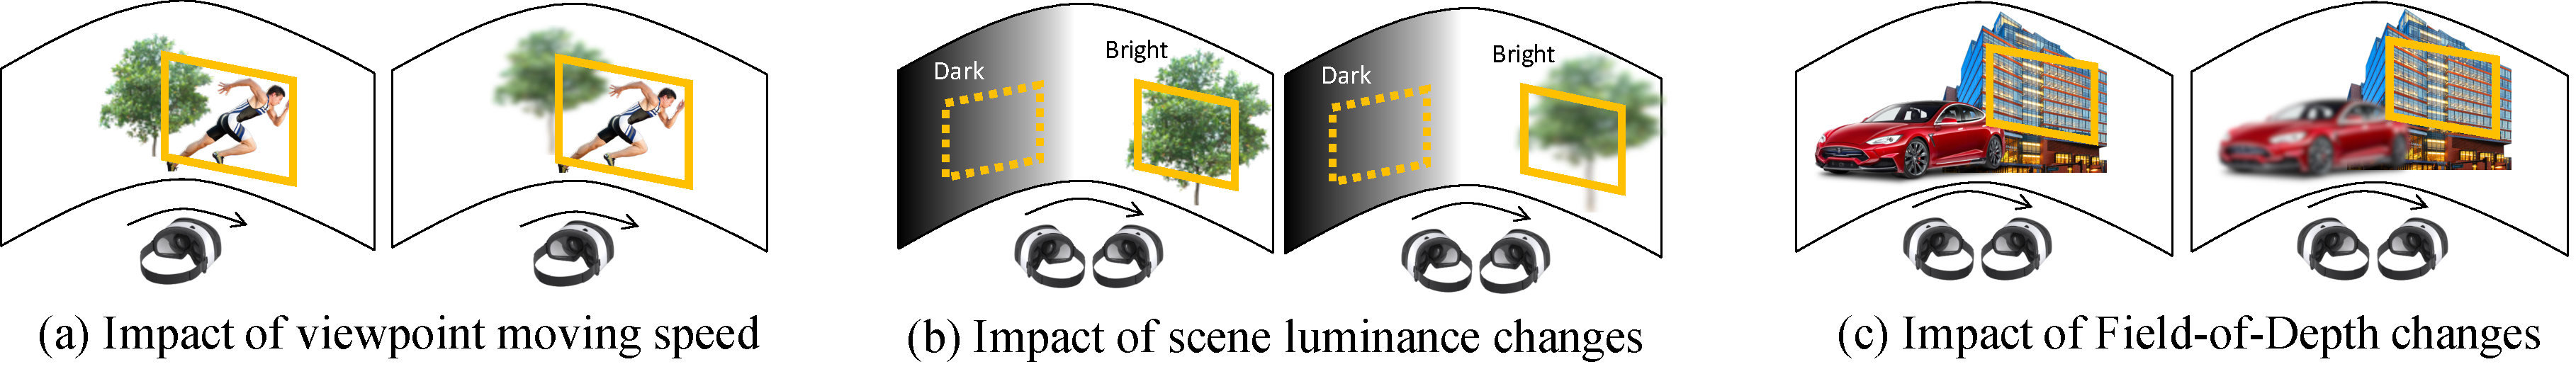
\includegraphics[width=0.9\textwidth]{figures/examples.pdf}
  \caption{Illustrative examples of the three \vr video-specific factor, and how they help save bandwidth by selectively reducing the quality of part of the video without affecting the user-perceived quality. The yellow boxes indicate the viewport (dashed ones are previous viewport). 
In each subgraph, the left-hand side and the right-hand side have similar perceived QoE, despite the quality distortions on some objects.}
  \label{fig:examples}
  \end{figure*}

We start with a background on \vrvideo streaming and today's common approach (\S\ref{subsec:background}, a full discussion on related work can be found in \S\ref{sec:related}).
Then, we outline several novel observations on user-perception of \vrvideo quality which inspire new opportunities to optimize the \vrvideo quality (\S\ref{subsec:opportunities}), and empiricially analyze their potential improvement for QoE (\S\ref{subsec:potentials}).
Finally, we highlight the challenges that must be addressed to unleash the potential benefits.


\subsection{Background of \vr video streaming}
\label{subsec:background}

%\mypara{\vr video streaming}
%\mypara{\vr videos coming to age}
%\vr video streaming is coming to age. 
By 2022, there will be over 55 million active VR headsets in the US, which is as many as paying Netflix members in the US in 2018~\cite{https://qz.com/1298512/vr-could-be-as-big-in-the-us-as-netflix-in-five-years-study-shows/}.
Almost all major content providers (YouTube~\cite{??}, Facebook~\cite{??}, Netflix~\cite{??}, Vimeo~\cite{??}, Amazon Prime~\cite{??}, Hulu~\cite{??}, iQIYI~\cite{??}, YouKu~\cite{??}) launched {\em streaming services for \vrvideos} on multiple  platforms~\cite{oculus,samsung,daydreams,etc}, believing that \vr videos are the future of story telling. 
\jc{add more concrete statistics on the popularity of VR}

%\mypara{Delivery architecture} 
The proliferation of the \vrvideo content and devices is also spurred by the highly efficient and scalable delivery architecture. 
Today, \vrvideos can be delivered to millions of concurrent viewers through commercial CDNs, in almost the same way non-\vr videos are delivered.
A \vrvideo is first encoded by a \vr encoder, which transcodes and chops the video into segments (or chunks); these video segments are then distributed to geo-distributed CDN edge servers; and finally, a client player (headset or smartphone) streams the video segments sequentially from the nearby CDN server using standard HTTP(S) (or DASH) protocols~\cite{hls,https://www.wowza.com/solutions/streaming-types/virtual-reality-and-360-degree-streaming}.
\jc{other than the client-side adaptation scheme, is there some fundamental diff or non-trivial steps involved in the preparation/dissemination of \vr content?}

To handle with last-mile bandwidth fluctuation, the video segments are encoded in multiple quality levels (usually quantization parameters or bitrates), and during playback, the \vrvideo player can switch quality level at the boundary between any two segments, in much the same way as non-\vr videos.
%Like non-\vr videos, \vrvideo streaming needs to cope with bandwidth fluctuation by adapting the quality level in order to strike a balance between video quality and bandwidth consumption.
%\mypara{Existing \vr video streaming protocols}
However, a distinctive feature of \vr video streaming is that the viewer's attention is {\em unevenly} distributed over a large area, with more attention centered around the viewport, whereas non-\vr videos are displayed on a fixed desktop or smartphone screen, os the unevenness of attention is less obvious.
Thus, \vrvideo streaming solutions also explore the {\em spatial} dimension: each video segment is spatially partitioned into tiles, each of which is encoded in multiple quality levels, so that different quality levels be used for different tiles depending on their {\em distance-to-viewport} ({\em DoV}), with higher quality in area closer to the user's viewpoint and lower quality for rest of the space.
This improves the perceived quality with the same or even less bandwidth consumption. 

%These {\em viewport-driven} protocols (\eg~\cite{??,??,??}) that the user-perceived quality of a spatial region is a function of the encoded quality and the region's distance to the viewport center.
Nevertheless, the gain of these {\em DoV-driven} protocols (\eg~\cite{??,??,??}) is limited, because the video segments must be short (typically one second, as opposed to 4-10 seconds in non-\vrvideos) so that the player can adapt the quality level as the viewpoint moves. \jc{add a concrete number for the size inflation due to the short chunk duration}
Despite many viewpoint-driven streaming~\cite{??,??,??} protocols or tiling mechanisms, this basic limit remains.



%\begin{figure}[t!]
%  \centering
%  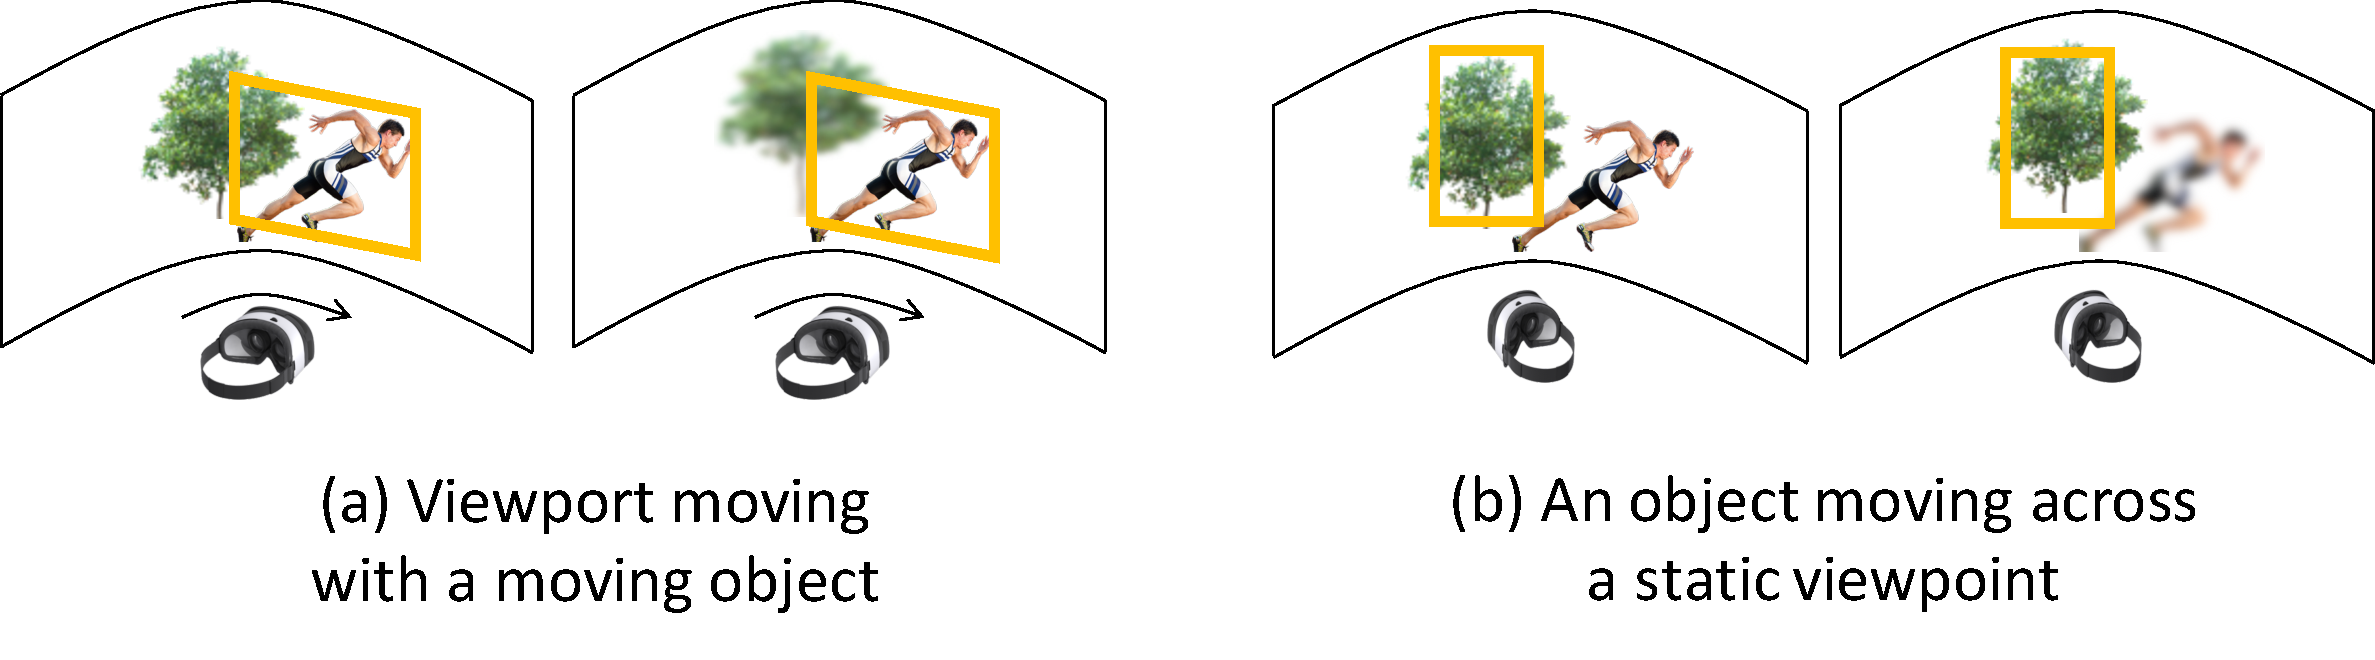
\includegraphics[width=0.5\textwidth]{figures/example-velocity.pdf}
%  \caption{Illustrative examples of the first \vr video-specific factor. 
%  Viewers tend to be insensitive to quality distortions of the objects moving at a high speed relative to the viewport, which can be (a) an object moving across a static viewport, or (b) the viewport moving across a static background. The yellow boxes indicate the viewport. 
%  In (a) and (b), the left-hand side and the right-hand side have similar perceived QoE, despite the quality distortions on some objects.}
%  \label{fig:example-velocity}
%  \end{figure}
%
%\begin{figure}[t!]
%  \centering
%  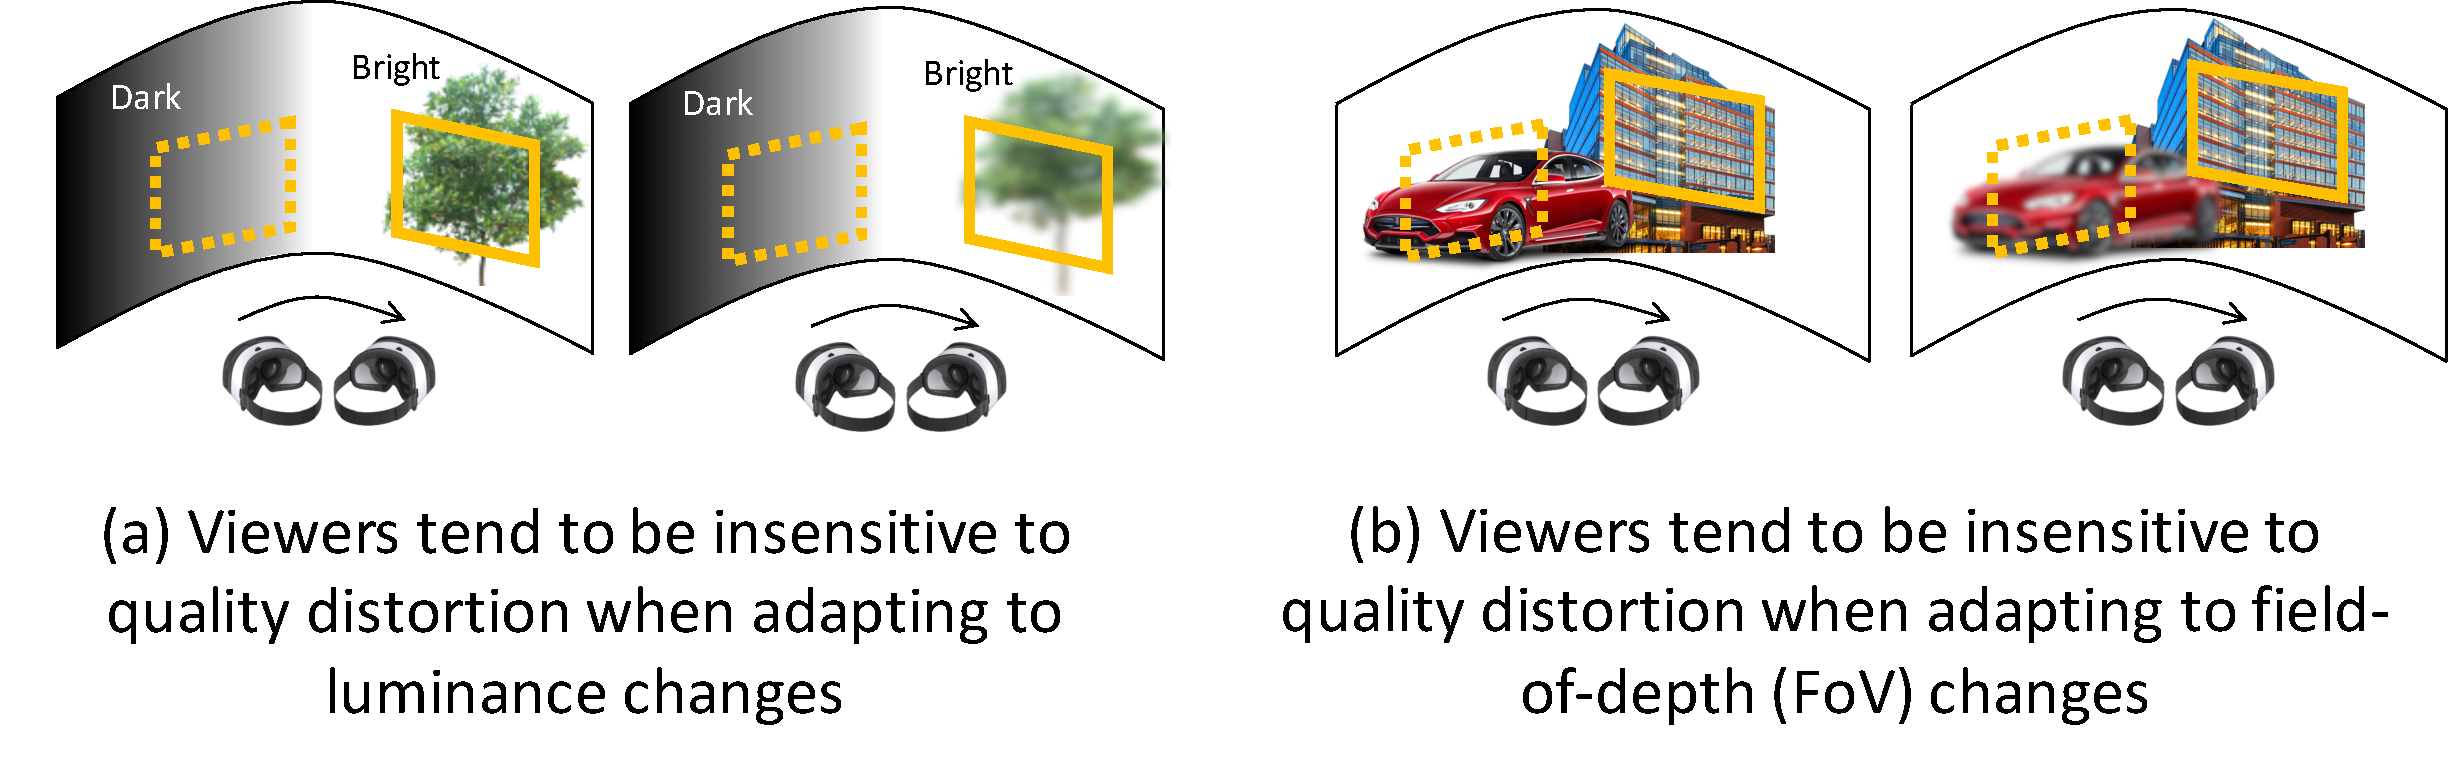
\includegraphics[width=0.5\textwidth]{figures/example-luminance-fov.pdf}
%  \caption{Illustrative examples of the 2nd and 3rd \vr video-specific factors. 
%  Viewers tend to be insensitive to quality distortions when (a) adapting to changes in luminance and when (b) an object has a different field-of-depth to the viewport.
%  The dashed boxes and solid boxes indicate where the viewport was and where it is now, respectively.
%  In both sub-figures, the left-hand side and the right-hand side have similar perceived QoE, despite the quality distortions on some objects.}
%  \label{fig:example-luminance}
%  \end{figure}

\subsection{New quality-determining factors}
\label{subsec:opportunities}

The driving intuition behind this work is that {\em through a deeper understanding of how viewers perceive \vrvideo quality, one can improve video quality or save bandwidth consumption without drop in perceived quality}.
Here, we briefly introduce three factors that can greatly affect the perceived quality of \vrvideos but have not been considered by existing \vrvideo streaming solutions. (\S\ref{sec:jnd} providers an in-depth analysis of these factors.)
%While the uneven distribution of the viewer's attention affects the QoE-bandwidth tradeoff, our first key observation is that it is just one of {\em several \vr video-specific factors that can heavily influence the perceived QoE of \vr videos but have yet to be fully explored}. 
%In particular, this paper examines the three following factors:

%\jc{need to visualize the three factors}

\begin{packeditemize}

%\myparashort
\item {\bf Factor\#1: Viewpoint moving speed.} 
%A key feature of \vr videos is that users can freely move their viewpoints. 
As the viewer moves her viewpoint, it also reduces the sensitivity to the quality distortion; and intuitively, the higher the speed, the lower the sensitivity. 
Figure~\ref{fig:examples}(a) gives an illustrative example of how this observation helps save bandwidth: when the viewer moves the viewpoint (\eg to track a moving object, as in the example), we found that reducing the quality level of static objects has little impact on user-perceived quality.
Similarly, when viewport is static, the viewer will tend to be insensitive to quality distortion of fast moving objects. 
%Consequently, as the viewers watch the video while moving their heads, they sometime report higher perceived quality than other static viewer perceive on the same video at the same objective quality level.
%the perceived quality is significantly improved, since user is unable to detect the distortion. 


%\myparashort
\item {\bf Factor\#2: Change in scene luminance.} 
Our second observation is that as the viewer moves her view around, the viewed region may switch between different levels of brightness, or luminance, and when the content changes from dark to bright (and vise versa), user's ability of detecting quality distortion also drops for a short period of time (typically \fillme seconds).
Figure~\ref{fig:examples}(b) illustrates a simple example of how one can carefully lower the quality level of part of the video without causing any drop in the user-perceived quality.
%When user wears a HMD in VR display, environmental brightness perceived by eyes is totally depended on luminance of video content itself.  
%As a result, when watching the same content encoded in the same objective quality, people report different levels of subjective quality depending on whether they have just watched something in different levels of luminance.


%\myparashort
\item {\bf Factor\#3: Differences in depth-of-field (DoF).} 
Our third observation is that a viewer can only be sensitive to the quality distortion of one of two objects, if they have different DoFs (\eg one being much closer to the viewer than the other).
Many \vr displays can precisely simulate the depths-of-field (DoF) by projecting an object to the two eyes with a specific binocular parallax (disparity) \jc{citation?}. 
Figure~\ref{fig:examples}(c) illustrates how one can reduce quality level of objects of different DoF than the object the viewer currently looks at\footnote{This paper assumes the object closest to the center of the viewport is the one watched by the viewer, which may not always hold. But this can be fixed if some gaze tracking mechanism (\eg~\cite{??,??}) is employed.}.
%We found that objects with small DoF (\ie closer to the viewer) have greater parallax, which lowers the viewer's sensitivity to quality distortion due to binocular fusion.
%As a result, a viewer might give different levels of attention to the objects of different DoF's, even if they are all close to the center of the viewport.

\end{packeditemize}
%\jc{why today's videos don't use them.}
We want to make two important remarks on these opportunities.

\myparaq{What is new about them}
While these factors (except DoF) have been studied in the context of traditional non-\vr videos, their benefits are greatly amplified in \vrvideo by the free viewpoint movements and the ability to track them. 
For instance, in non-\vr videos, fast-moving parts of the video may be given lower quality than static parts, but \vrvideos open up new opportunities as the viewer may actually look at the moving object, thus one can use lower quality for the whole background. 
On the other hand, these factors are certainly different to traditional viewpoint-driven streaming adaptation, which assumes the user-perceived quality only depends on the distance-to-viewpoint. 


\mypara{Intuitive explanation}
The key intuition behind all these opportunities is that {\em each viewer has a limited span of attention}.
With the new features of panoramic view and immersive experience, the video size grow dramatically, but the span of attention remains largely constant\footnote{The span of attention does grow as the \vr headset shows a bigger virtual screen, but this is a much smaller increase compared to the size inflation of the whole \vrvideo.}. 
Consequently, a viewer will give less attention to the specifics of a \vr video, which in turn reduces the sensitivity to the quality distortion at some parts of the video, creating a multitude of room for improving the bandwidth-QoE tradeoffs, including viewport-driven adaptation as well as the three aforementioned factors.


%\jc{
%\begin{itemize}
%\item p1: we first extend the jnd model with several \vr specific factors, 1, 2, 3
%\item p2: with the new jnd model (explained latter), the potential improvement is tremendous!
%\end{itemize}
%}




%The uneven distribution of \vr user's sensitivities can be explained by the attention theory~\cite{??,??}, which has been successfully applied to specialized video encoder and human-computer interface. 
%The key concept is the just-noticeable difference (JND)---a user tends to notice the difference between two images/videos, only after the difference is greater than a threshold of JND, which depends heavily on the image/video content (as well as the context of the viewer).
%\jc{add a few examples of JND, like content luminance, texture complexity}

%The existing viewport-driven streaming protocols can be seen as one design point of using JND which only depends on the distance between a region and the viewport center. 
%We have seen a few efforts to introduce the existing JND-based attention models in video streaming~\cite{??,??}, although so far their real application so far has been quite limited.


\subsection{Potential for improvement}
\label{subsec:potentials}

Next, we use a real-world dataset to analyze the potential practical QoE improvement and bandwidth savings of the new opportunities. 


\begin{table}[t]
\begin{tabular}{rc}
 \hline
Videos & \fillme \\ \hline
Original resolution & \fillme by \fillme \\ \hline
Duration & \fillme$\sim$\fillme minutes \\ \hline
Views per video & \fillme \\ \hline
\end{tabular}
\caption{Dataset summary}
\label{tab:dataset}
\end{table}


\mypara{Dataset}
The dataset consists of \fillme \vrvideos, each watched by \fillme users.
The video dataset was provided by \fillme\jc{what's the source?}, and can be found in \fillme \jc{is there a public source?}
Each video was played by a \fillme device~\cite{??}
The video content covers three major categories: sports (\fillme), movies (\fillme), theater (\fillme).
Table~\ref{tab:dataset} gives a summary of the dataset.

\myparaq{How prevalent are these factors}
We first measure the prevalence of these new factors. 
Figure~\ref{fig:prevalence} shows the distribution of viewpoint-moving speed, luminance changes in a small time window, and DoF differences among objects in the viewport (which will not be differentiated by existing techniques).
We can see that they all occur for a substantial fraction of times. 
For instance, for more than 30\% of time, the viewpoint is moving faster than 20~degree/s. 
To put it into perspective, this means 30\% of time, the viewers are unlikely to perceive a \fillme\% drop in quality of the static background content (as we will show in \S\ref{subsec:??}).
Similarly, \jc{a sentence on the other two graphs.}


%%According to our data analysis, more than \fillme\% time, user's viewpoint is moving faster than \fillme \textdegree/s. 
%One of the most highlighted feature of VR video is that users can freely move their viewpoints. According to our data analysis, more than 30\% viewpoints are moving faster than 20 deg/s. (Fig. \ref{CDFspeed}) 
%When human viewpoint is moving, visual acuity is decreased in 2 different conditions: (1) if user is tracking an object, visual acuity decreases smoothly with viewpoint moving speed increases. (2) If user is not tracking an object, visual acuity decreases dramatically with viewpoint moving speed increases. \cite{speed}
%\jc{can you visualize such findings, and also show some numbers about the other two factors?}

\begin{figure}
  \centering
  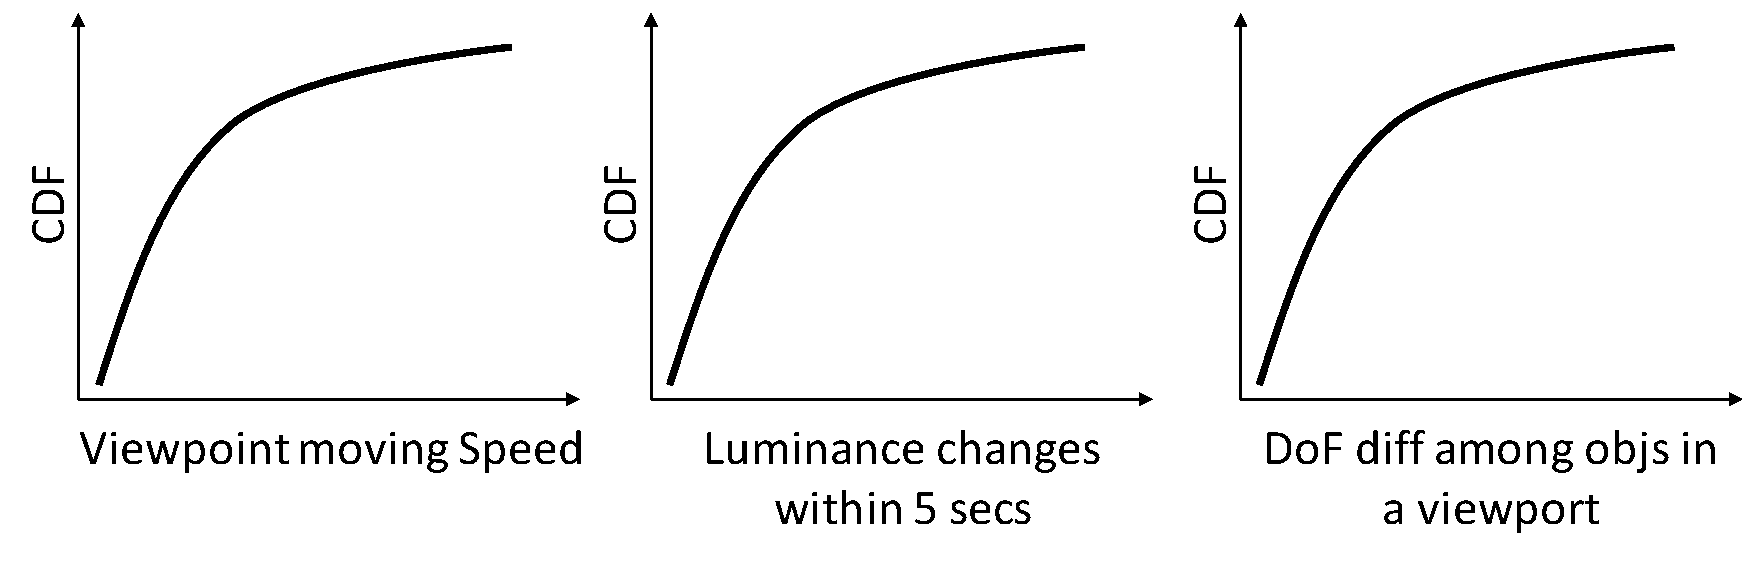
\includegraphics[width=0.5\textwidth]{figures/prevalence.pdf}
  \caption{Prevalence of the new opportunities.}
  \label{fig:prevalence}
 \end{figure}



\mypara{Potential gains in quality-bandwidth tradeoffs}
To show the practical benefits of these new factors in improving video quality, we consider an idealized scheme for encoding a \vrvideo, called {\em idealized \vrvideo}.
\jc{need details, how many quality levels? how many tiles? how to allocate quality levels under a given bandwidth?}
We compare it with a baseline inspired by the common DoV-driven approach: each frame is split into 
6*12 equal-sized rectangular tiles\footnote{\jc{how do we handle the problem of curved sphere? did we use any standard techniques?}}, and the tile covering the viewport are given the highest quality level, \jc{and how to allocate the rest tiles?}

Figure~\ref{fig:potential} shows that the idealized \vrvideo achieves a much better quality-bandwidth tradeoffs than the DoV-driven baseline.
We use peak signal-to-perceptible-noise ratio (PSPNR)~\cite{??} as an indicator of the perceived quality. 
We will discuss PSPNR in full details in \S\ref{sec:jnd}, but in short, it has a stronger linear correlation to subjective user rating than alternative measures (\eg PSNR).
The idealized \vrvideo can save \fillme\% bandwidth without drop in PSPNR, or improve PSPNR by \fillme\% (roughly an \fillme\% increase in user rating) using the same amount of bandwidth.

It should be noticed that both schemes are idealized since the viewpoint trajectory cannot be known in advance, but their comparison is indicative of the actual performance difference between the practical solutions. 

%Before giving the concrete design of an actual streaming protocol, we first present the potential for improvement of leveraging the \vr-specific factors. 
%To do so, we use a metric called PSPNR to denote the perceived quality of a viewer, which can be expressed by $F(P,P',A,v,d,\Delta d,l,\Delta l)$, where $P$ and $P'$ denote the original frame and the rendered frame respectively, $a=(x_a,y_a)$ the viewport center, $v$ the viewport moving speed, $d$ the DoF, $\Delta d$ the change in DoF, $l$ the luminance, and $\Delta l$ the change in luminance. 
%We will explain this metric in greater detail in the next section. 
%\jc{give a short description of how to understand PSPNR}

%PSPNR \cite{PSPNR} is applied as a metric to measure perceived quality. Real traces are collected from over 800 VR displays of 48 users. In our experiment, each video has 5 different bitrate level. We compare the performance of 3 methods:
%\begin{itemize}
%
%\item \emph{Viewpoint-driven VR streaming.} Video is cut into 6*12 spatial rectangular tiles. Tiles on user's viewpoint is allocated the high bitrate. For other tiles, bitrate is allocated linearly decreasing with its distance to user's viewpoint.
%
%\item \emph{Perceived quality driven VR streaming. (with 3 VR factors)} Suppose we can freely allocate bitrate to each spatial part of video without video tiling. Besides user viewpoint, content luminance and texture complexity, we also take consideration of viewpoint moving speed, content Depth-of-Field and light / dark adaptation, we do adaptive streaming to maximize user-perceived quality.
%
%\end{itemize}
%
%With consideration of content luminance and texture complexity, perceived-quality-driven VR streaming can save 30\% bandwidth compared with viewpoint-driven VR streaming providing the same PSPNR. Moreover, when we take consideration of viewpoint moving speed, object Depth-of-Field and light / dark adaptation, we can further save 20\% bandwidth.


\begin{figure}
  \centering
  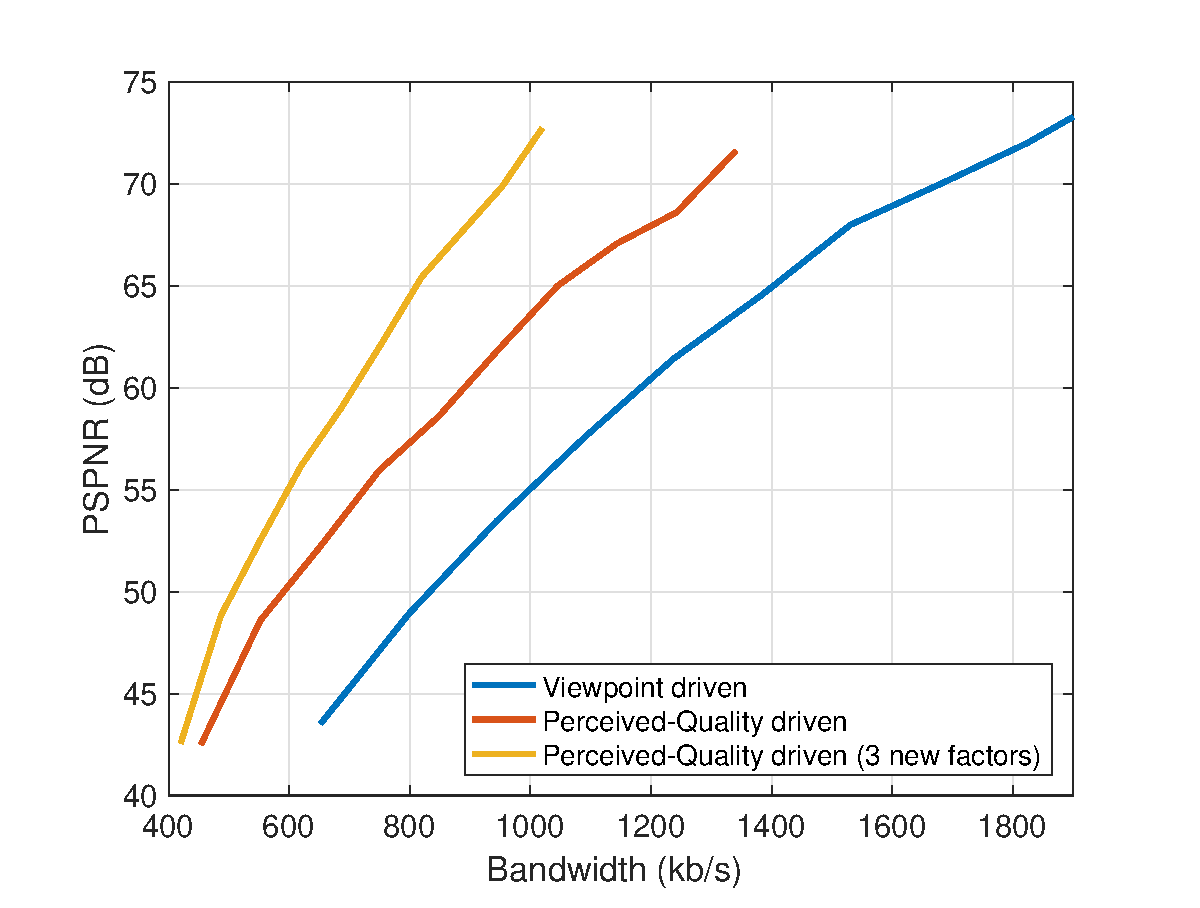
\includegraphics[width=2.5in]{images/improvement.eps}
  \caption{PSPNR-bandwidth tradeoff of (1) Viewpoint-driven VR streaming. (2) Perceived quality driven VR streaming. (3) Perceived quality driven VR streaming. (with 3 VR factors)}
  \label{fig:potential}
  \end{figure}




\subsection{Key challenges}

However, to fully explore these opportunities requires not only changing the quality objective function, but re-architecting several critical components of the video delivery pipeline. 
In particular, we identify three main challenges.

%In order to achieve perceived quality driven VR streaming, the core challenge is: perceived quality is related to both video content and user behavior, how to take together both-sides information to maximize the perceived quality. For specifically, there are three aspects:

\myparashort{Challenge 1: How to leverage the new quality-determining factors in \vrvideo streaming?}
%Challenge 1: Traditional Human Visual System (HVS) models can not measure perceived quality in VR video display.
Before designing the streaming protocol, we first need to incorporate the new quality-determining factors to how \vrvideo quality is measured. 
This, however, is not trivial, as most traditional video quality metrics focus on the impact of content-level dynamism (\eg users are relatively insensitive to quality distortion on a ``busy'' scene) while assuming the viewers are static.
On the contrary, the new quality-determining factors are driven mostly by user actions. 
So our first step is to incorporate them in existing video quality metrics.
%Perceived quality can be well-measured in traditional video display by building mathematical model from luminance, texture complexity and viewpoint-object distance to perceived quality. However, as we have mentioned, besides these existing factors, perceived quality in VR display is related to several new factors which are never modeled before. Their mathematical relationship to perceived quality, and how these new factors combined with existing factors together influence perceived quality are unknown problems.

\myparashort{Challenge 2: How should the \vrvideos be spatially tiled to fully exploit the new opportunities?}
%Challenge 2: Traditional grid-like video tiling scheme performs poorly in perceived quality optimization.
Second, the spatial tiling of \vrvideos must allow enough flexibility so that the quality adaptation logic can differentiate spatial regions to which the viewer has different sensitivity. 
For instance, it is ideal if the tiling is such that objects moving at different speed (\eg foreground vs background) can be assigned with different quality levels.
At a first glance, this can be done by using more fine-grained tiling, but this is not practical as finer-grained tiling will inevitably reduce video  coding efficiency and thus drastically inflate the bandwidth consumption.
Figure~\ref{fig:bitrate-efficiency} shows the average size inflation of all videos in the dataset (the tiled video size over the original video size), and that the size grows almost linearly with the number of tiles. 
So the existing equal-sized tiling mechanism is not sufficient to fully explore the new opportunities.

%To optimize perceived quality, we need to independently allocate bitrate of each spatial part of the video. Grid-like tiling scheme is a widely used method to solve the problem. Video is cut into several rectangular tiles with equal size which can be independently encoded / decoded. So we can allocate different bitrate to different tiles.
%
%However, traditional grid-like tiling performs poorly in perceived quality optimization in two aspects: 
%
%(1) Coarse-grained tiling causes coarse-grained rate allocation, and perceived quality obtained by coarse-grained rate allocation is far from that obtained by fine-grained rate allocation. We encode the video with different rate allocation granularity. We apply PSPNR to measure perceived quality and Fig. \ref{optimalencoding} shows the PSPNR-bandwidth tradeoff. Rate allocation with 3*6 / 6*12 granularity obtains -x\% / -x\% PSPNR compared with 12*24 granularity, this is a significant performance gap in perceived quality optimization.
%
%\begin{figure}
%  \centering
%  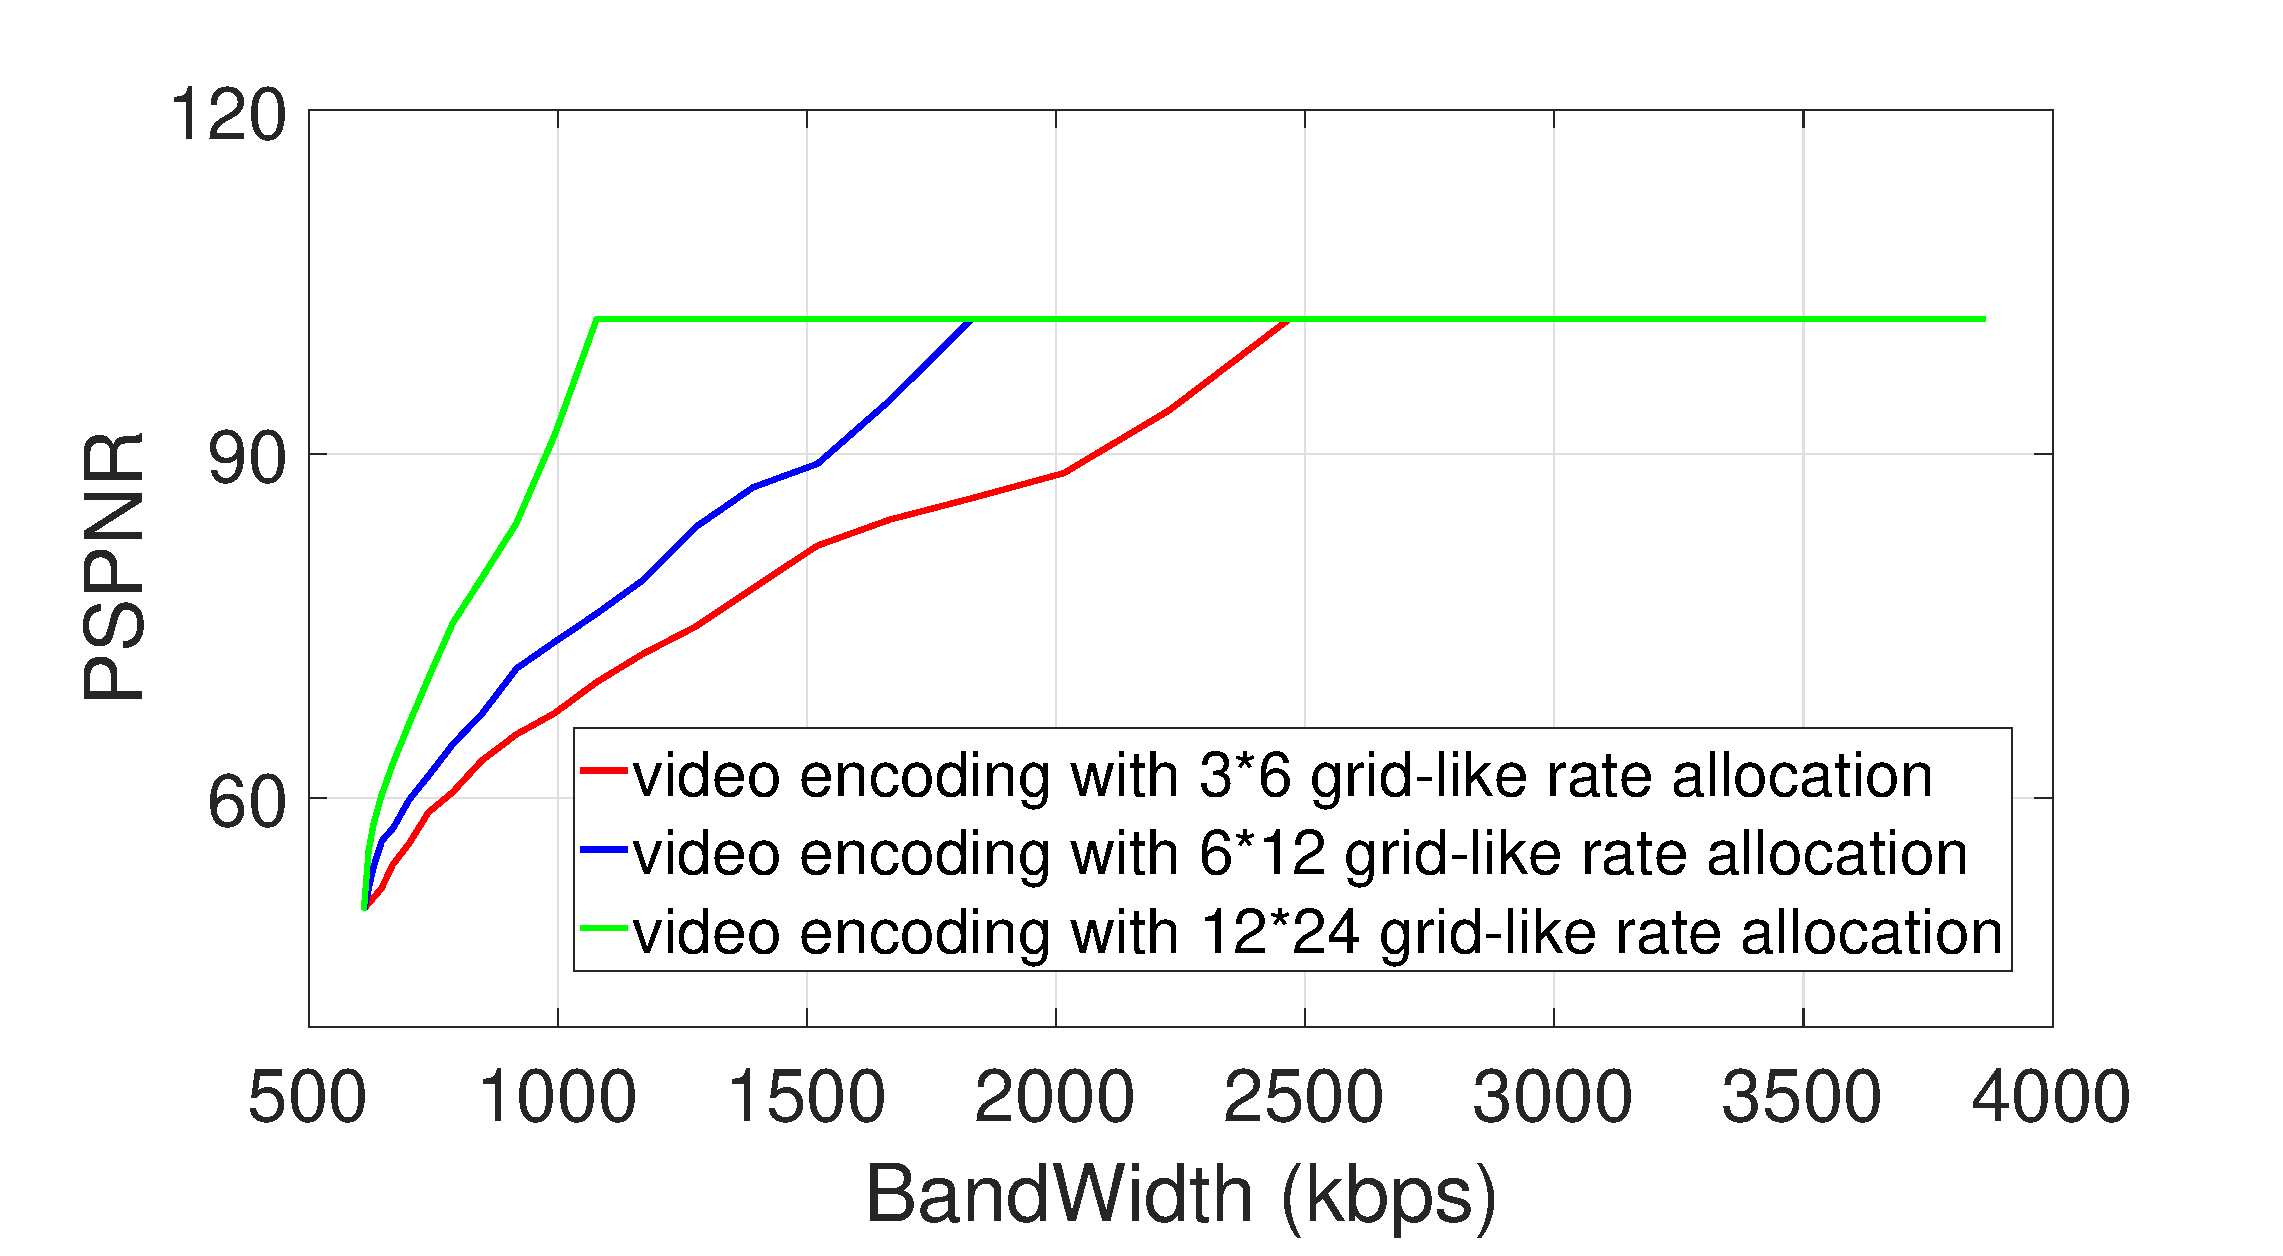
\includegraphics[width=2.5in]{images/optimalencoding.eps}
%  \caption{PSPNR-bandwidth tradeoff in video encoding with different granularity of rate allocation.}
%  \label{optimalencoding}
%  \end{figure}
%
%(2) Fine-grained tiling introduces serious bitrate efficiency problem in video encoding. In practice, each tile has to be encoded independently instead of encoded together. When we cut the video into tiles, the total video size is increased. Fig. \ref{bitrateefficiency} shows the video size of different tiling granularity compared with original video size. We find that cutting a video into 12*24 tiles introduces 50\% to 330\% additional video size compared to original video. This significantly lower its practical performance in perceived quality optimization, especially in low bandwidth situations where the bitrate efficiency problem is very serious.

\begin{figure}
  \centering
  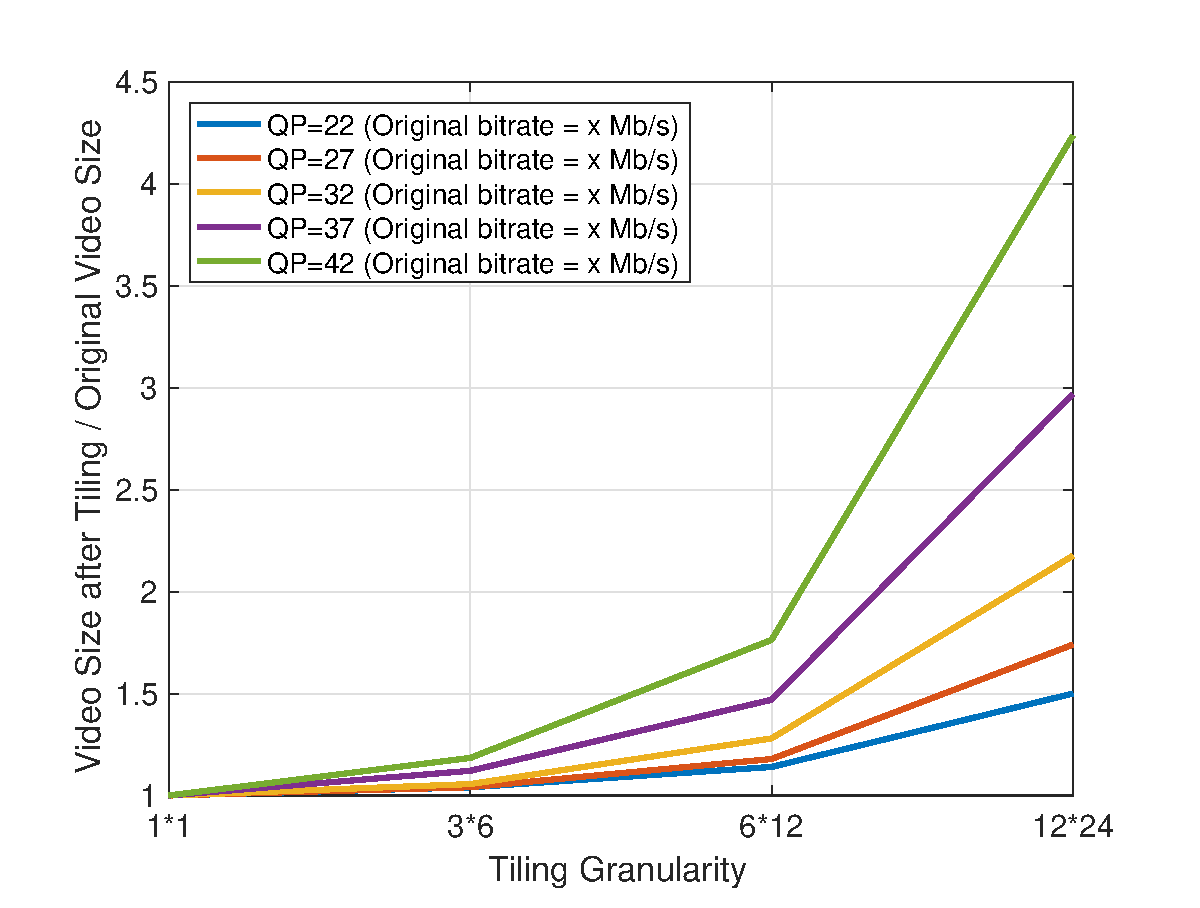
\includegraphics[width=2.5in]{images/bitrateefficiency.eps}
  \caption{The ratio of video size after tiling and original video size in each tiling granularity and each bitrate level. We notice that fine-grained tiling introduces serious bitrate efficiency problem, especially in low bandwidth situations in which the overall bitrate of each tile is low. \jc{pick one line. no need for five lines}}
  \label{fig:bitrate-efficiency}
  \end{figure}

\myparashort{Challenge 3: How to design a streaming protocol that is robust to noises in user action and compatible with the existing delivery infrastructure?}
%Challenge 3: Information needed for perceived quality computation is disparted on server-side and client-side.
Finally, the new quality-determining factors call for a revisit on the streaming protocol. 
On one hand, it seems the protocol must be sufficiently adaptive to cope not just fluctuation in bandwidth variation and viewpoint movement, but also real-time changes of the movement velocity, the scene luminance, and the depth-of-field. 
On the other hand, the streaming protocol must also be architecturally compatible with the HTTP-based delivery infrastructure that has spurred the rise of \vrvideos, so the quality adaptation is driven solely by the client (while the server passively server the video as web objects). 
Unfortunately, this is difficult because, as we will see, to calculate the optimal quality level, the client needs the knowledge of the video content before streaming the content. 

%To optimize perceived quality, client needs to compute the perceived quality of each bitrate allocation and then make decision. However, different from video quality which only related to video content itself, perceived quality depends on both video content and user behavior. Information of video content is located on server-side while information of user behavior is located on client-side. To get information of video content with current DASH, client has to pre-request in information of each pixel from server. This communication overload even exceed the overload of actual video streaming.



